% Options for packages loaded elsewhere
\PassOptionsToPackage{unicode}{hyperref}
\PassOptionsToPackage{hyphens}{url}
%
\documentclass[
  8pt,
  ignorenonframetext,
]{beamer}
\usepackage{pgfpages}
\setbeamertemplate{caption}[numbered]
\setbeamertemplate{caption label separator}{: }
\setbeamercolor{caption name}{fg=normal text.fg}
\beamertemplatenavigationsymbolsempty
% Prevent slide breaks in the middle of a paragraph
\widowpenalties 1 10000
\raggedbottom
\setbeamertemplate{part page}{
  \centering
  \begin{beamercolorbox}[sep=16pt,center]{part title}
    \usebeamerfont{part title}\insertpart\par
  \end{beamercolorbox}
}
\setbeamertemplate{section page}{
  \centering
  \begin{beamercolorbox}[sep=12pt,center]{part title}
    \usebeamerfont{section title}\insertsection\par
  \end{beamercolorbox}
}
\setbeamertemplate{subsection page}{
  \centering
  \begin{beamercolorbox}[sep=8pt,center]{part title}
    \usebeamerfont{subsection title}\insertsubsection\par
  \end{beamercolorbox}
}
\AtBeginPart{
  \frame{\partpage}
}
\AtBeginSection{
  \ifbibliography
  \else
    \frame{\sectionpage}
  \fi
}
\AtBeginSubsection{
  \frame{\subsectionpage}
}
\usepackage{amsmath,amssymb}
\usepackage{lmodern}
\usepackage{iftex}
\ifPDFTeX
  \usepackage[T1]{fontenc}
  \usepackage[utf8]{inputenc}
  \usepackage{textcomp} % provide euro and other symbols
\else % if luatex or xetex
  \usepackage{unicode-math}
  \defaultfontfeatures{Scale=MatchLowercase}
  \defaultfontfeatures[\rmfamily]{Ligatures=TeX,Scale=1}
\fi
% Use upquote if available, for straight quotes in verbatim environments
\IfFileExists{upquote.sty}{\usepackage{upquote}}{}
\IfFileExists{microtype.sty}{% use microtype if available
  \usepackage[]{microtype}
  \UseMicrotypeSet[protrusion]{basicmath} % disable protrusion for tt fonts
}{}
\makeatletter
\@ifundefined{KOMAClassName}{% if non-KOMA class
  \IfFileExists{parskip.sty}{%
    \usepackage{parskip}
  }{% else
    \setlength{\parindent}{0pt}
    \setlength{\parskip}{6pt plus 2pt minus 1pt}}
}{% if KOMA class
  \KOMAoptions{parskip=half}}
\makeatother
\usepackage{xcolor}
\newif\ifbibliography
\usepackage{color}
\usepackage{fancyvrb}
\newcommand{\VerbBar}{|}
\newcommand{\VERB}{\Verb[commandchars=\\\{\}]}
\DefineVerbatimEnvironment{Highlighting}{Verbatim}{commandchars=\\\{\}}
% Add ',fontsize=\small' for more characters per line
\usepackage{framed}
\definecolor{shadecolor}{RGB}{248,248,248}
\newenvironment{Shaded}{\begin{snugshade}}{\end{snugshade}}
\newcommand{\AlertTok}[1]{\textcolor[rgb]{0.94,0.16,0.16}{#1}}
\newcommand{\AnnotationTok}[1]{\textcolor[rgb]{0.56,0.35,0.01}{\textbf{\textit{#1}}}}
\newcommand{\AttributeTok}[1]{\textcolor[rgb]{0.77,0.63,0.00}{#1}}
\newcommand{\BaseNTok}[1]{\textcolor[rgb]{0.00,0.00,0.81}{#1}}
\newcommand{\BuiltInTok}[1]{#1}
\newcommand{\CharTok}[1]{\textcolor[rgb]{0.31,0.60,0.02}{#1}}
\newcommand{\CommentTok}[1]{\textcolor[rgb]{0.56,0.35,0.01}{\textit{#1}}}
\newcommand{\CommentVarTok}[1]{\textcolor[rgb]{0.56,0.35,0.01}{\textbf{\textit{#1}}}}
\newcommand{\ConstantTok}[1]{\textcolor[rgb]{0.00,0.00,0.00}{#1}}
\newcommand{\ControlFlowTok}[1]{\textcolor[rgb]{0.13,0.29,0.53}{\textbf{#1}}}
\newcommand{\DataTypeTok}[1]{\textcolor[rgb]{0.13,0.29,0.53}{#1}}
\newcommand{\DecValTok}[1]{\textcolor[rgb]{0.00,0.00,0.81}{#1}}
\newcommand{\DocumentationTok}[1]{\textcolor[rgb]{0.56,0.35,0.01}{\textbf{\textit{#1}}}}
\newcommand{\ErrorTok}[1]{\textcolor[rgb]{0.64,0.00,0.00}{\textbf{#1}}}
\newcommand{\ExtensionTok}[1]{#1}
\newcommand{\FloatTok}[1]{\textcolor[rgb]{0.00,0.00,0.81}{#1}}
\newcommand{\FunctionTok}[1]{\textcolor[rgb]{0.00,0.00,0.00}{#1}}
\newcommand{\ImportTok}[1]{#1}
\newcommand{\InformationTok}[1]{\textcolor[rgb]{0.56,0.35,0.01}{\textbf{\textit{#1}}}}
\newcommand{\KeywordTok}[1]{\textcolor[rgb]{0.13,0.29,0.53}{\textbf{#1}}}
\newcommand{\NormalTok}[1]{#1}
\newcommand{\OperatorTok}[1]{\textcolor[rgb]{0.81,0.36,0.00}{\textbf{#1}}}
\newcommand{\OtherTok}[1]{\textcolor[rgb]{0.56,0.35,0.01}{#1}}
\newcommand{\PreprocessorTok}[1]{\textcolor[rgb]{0.56,0.35,0.01}{\textit{#1}}}
\newcommand{\RegionMarkerTok}[1]{#1}
\newcommand{\SpecialCharTok}[1]{\textcolor[rgb]{0.00,0.00,0.00}{#1}}
\newcommand{\SpecialStringTok}[1]{\textcolor[rgb]{0.31,0.60,0.02}{#1}}
\newcommand{\StringTok}[1]{\textcolor[rgb]{0.31,0.60,0.02}{#1}}
\newcommand{\VariableTok}[1]{\textcolor[rgb]{0.00,0.00,0.00}{#1}}
\newcommand{\VerbatimStringTok}[1]{\textcolor[rgb]{0.31,0.60,0.02}{#1}}
\newcommand{\WarningTok}[1]{\textcolor[rgb]{0.56,0.35,0.01}{\textbf{\textit{#1}}}}
\usepackage{graphicx}
\makeatletter
\def\maxwidth{\ifdim\Gin@nat@width>\linewidth\linewidth\else\Gin@nat@width\fi}
\def\maxheight{\ifdim\Gin@nat@height>\textheight\textheight\else\Gin@nat@height\fi}
\makeatother
% Scale images if necessary, so that they will not overflow the page
% margins by default, and it is still possible to overwrite the defaults
% using explicit options in \includegraphics[width, height, ...]{}
\setkeys{Gin}{width=\maxwidth,height=\maxheight,keepaspectratio}
% Set default figure placement to htbp
\makeatletter
\def\fps@figure{htbp}
\makeatother
\setlength{\emergencystretch}{3em} % prevent overfull lines
\providecommand{\tightlist}{%
  \setlength{\itemsep}{0pt}\setlength{\parskip}{0pt}}
\setcounter{secnumdepth}{-\maxdimen} % remove section numbering
\ifLuaTeX
  \usepackage{selnolig}  % disable illegal ligatures
\fi
\IfFileExists{bookmark.sty}{\usepackage{bookmark}}{\usepackage{hyperref}}
\IfFileExists{xurl.sty}{\usepackage{xurl}}{} % add URL line breaks if available
\urlstyle{same} % disable monospaced font for URLs
\hypersetup{
  pdftitle={intro to programming 5},
  pdfauthor={Henri Vandendriessche},
  hidelinks,
  pdfcreator={LaTeX via pandoc}}

\title{intro to programming 5}
\author{Henri Vandendriessche}
\date{19/10/2021}

\begin{document}
\frame{\titlepage}

\begin{frame}{So far}
\protect\hypertarget{so-far}{}
\begin{itemize}
\item
  Python, its life, its choice
\item
  Data types: (integer / float / string / boolean)
\item
  \textbf{If}, \textbf{For} and \textbf{While} loops:
\item
  Data collections: (list, tuple, set, dictionary)
\item
  Functions
\item
  Higher order function (Recursive function)
\end{itemize}
\end{frame}

\begin{frame}{Today}
\protect\hypertarget{today}{}
\begin{block}{- Read and write files}
\protect\hypertarget{read-and-write-files}{}
\end{block}
\end{frame}

\begin{frame}{Manipulate files : Open and read a file 1/3}
\protect\hypertarget{manipulate-files-open-and-read-a-file-13}{}
\begin{itemize}
\item
  To do so you have one function available in the built-in functions of
  python

  \begin{itemize}
  \tightlist
  \item
    \url{https://docs.python.org/3/library/functions.html}
  \end{itemize}
\item
  The function \textbf{open()}

  \begin{itemize}
  \tightlist
  \item
    that works like that open(file, mode=`r', buffering=- 1,
    encoding=None, errors=None, newline=None, closefd=True, opener=None)
  \end{itemize}
\item
  see \url{https://docs.python.org/3/library/functions.html\#open}
\item
  Mode can be:

  \begin{itemize}
  \tightlist
  \item
    ``r'' - Read - Default value. Opens a file for reading, error if the
    file does not exist
  \item
    ``a'' - Append - Opens a file for appending, creates the file if it
    does not exist
  \item
    ``w'' - Write - Opens a file for writing, creates the file if it
    does not exist
  \item
    ``x'' - Create - Creates the specified file, returns an error if the
    file exist
  \end{itemize}
\end{itemize}
\end{frame}

\begin{frame}[fragile]{Manipulate files : Open and read a file 2/3}
\protect\hypertarget{manipulate-files-open-and-read-a-file-23}{}
\begin{itemize}
\item
  to manipulate and for example print the text you need to read it using
  \textbf{read()}
\item
  All available function are specified here:

  \begin{itemize}
  \tightlist
  \item
    \url{https://docs.python.org/3/library/io.html}
  \end{itemize}
\end{itemize}

\begin{Shaded}
\begin{Highlighting}[]
\NormalTok{Myfile }\OperatorTok{=} \BuiltInTok{open}\NormalTok{(}\StringTok{\textquotesingle{}Survival rules for programming.txt\textquotesingle{}}\NormalTok{, }\StringTok{\textquotesingle{}r\textquotesingle{}}\NormalTok{)}
\BuiltInTok{print}\NormalTok{(Myfile.read())}
\end{Highlighting}
\end{Shaded}

\begin{verbatim}
## Try by yourself before looking for solutions
## 
## Internet is your best friend
## 
## Read the manual
## 
## There is always a manual
## 
## Have you read the fucking manual?
## 
## Not yet ? Then read it
## 
## Always read the error message
\end{verbatim}

\begin{Shaded}
\begin{Highlighting}[]
\BuiltInTok{print}\NormalTok{(Myfile.read(}\DecValTok{5}\NormalTok{))}
\end{Highlighting}
\end{Shaded}

\begin{Shaded}
\begin{Highlighting}[]
\NormalTok{Myfile.close()}
\end{Highlighting}
\end{Shaded}
\end{frame}

\begin{frame}[fragile]{Manipulate files : Open and read a file 3/3}
\protect\hypertarget{manipulate-files-open-and-read-a-file-33}{}
\begin{itemize}
\item
  You can also use:
\item
  readline() can be used to return one line
\item
  readlines() can be used to return a list of lines
\item
  NB 1: if the file is not close the next call of readline() or
  readlines() will take the subsequent lines of the file even though you
  specified the first index
\item
  NB 2: As readlines() return a list you can use all the functions in
  the built in module \textbf{string} such as len(), joins(),
  split()\ldots{}
\end{itemize}

\begin{Shaded}
\begin{Highlighting}[]
\NormalTok{Myfile }\OperatorTok{=} \BuiltInTok{open}\NormalTok{(}\StringTok{\textquotesingle{}Survival rules for programming.txt\textquotesingle{}}\NormalTok{, }\StringTok{\textquotesingle{}r\textquotesingle{}}\NormalTok{)}
\BuiltInTok{print}\NormalTok{(Myfile.readline())}
\end{Highlighting}
\end{Shaded}

\begin{verbatim}
## Try by yourself before looking for solutions
\end{verbatim}

\begin{Shaded}
\begin{Highlighting}[]
\BuiltInTok{print}\NormalTok{(Myfile.readlines(}\DecValTok{1}\NormalTok{))}
\end{Highlighting}
\end{Shaded}

\begin{verbatim}
## ['\n', 'Internet is your best friend\n']
\end{verbatim}

\begin{Shaded}
\begin{Highlighting}[]
\BuiltInTok{print}\NormalTok{(Myfile.readlines()[}\DecValTok{1}\NormalTok{])}
\end{Highlighting}
\end{Shaded}

\begin{verbatim}
## Read the manual
\end{verbatim}
\end{frame}

\begin{frame}[fragile]{Manipulate files : create a file}
\protect\hypertarget{manipulate-files-create-a-file}{}
\begin{itemize}
\tightlist
\item
  Note that if you don't specify any path, it will be created in the
  current directory (ie, same directory as your script). It's called
  creating a file using a \textbf{relative path}
\end{itemize}

\begin{Shaded}
\begin{Highlighting}[]
\ImportTok{import}\NormalTok{ os}
\NormalTok{path }\OperatorTok{=}\NormalTok{ os.getcwd()}

\BuiltInTok{print}\NormalTok{(os.listdir(path))}
\end{Highlighting}
\end{Shaded}

\begin{verbatim}
## ['intro-to-programming-5.Rmd', 'intro-to-programming-5.html', 'Survival rules for programming.txt', 'hist.png']
\end{verbatim}

\begin{Shaded}
\begin{Highlighting}[]
\NormalTok{MyTestFile }\OperatorTok{=} \BuiltInTok{open}\NormalTok{(}\StringTok{\textquotesingle{}test.txt\textquotesingle{}}\NormalTok{, }\StringTok{\textquotesingle{}x\textquotesingle{}}\NormalTok{)}

\BuiltInTok{print}\NormalTok{(os.listdir(path))}
\end{Highlighting}
\end{Shaded}

\begin{verbatim}
## ['test.txt', 'intro-to-programming-5.Rmd', 'intro-to-programming-5.html', 'Survival rules for programming.txt', 'hist.png']
\end{verbatim}

\begin{itemize}
\tightlist
\item
  If you want to create in a precise directory you can specify it using
  an \textbf{absolute path}
\end{itemize}

\begin{Shaded}
\begin{Highlighting}[]
\NormalTok{MyTestFile }\OperatorTok{=} \BuiltInTok{open}\NormalTok{(}\StringTok{\textquotesingle{}/home/henri/Desktop/test.txt\textquotesingle{}}\NormalTok{, }\StringTok{\textquotesingle{}x\textquotesingle{}}\NormalTok{)}
\end{Highlighting}
\end{Shaded}
\end{frame}

\begin{frame}[fragile]{Manipulate files : write a file}
\protect\hypertarget{manipulate-files-write-a-file}{}
\begin{itemize}
\item
  We need an access mode `w' if we want to create and write anything
  into a file
\item
  Note that to be able to read a just created file you need to close it
  and open it again in read mode
\end{itemize}

\begin{Shaded}
\begin{Highlighting}[]
\NormalTok{MyTestFile }\OperatorTok{=} \BuiltInTok{open}\NormalTok{(}\StringTok{\textquotesingle{}test2.txt\textquotesingle{}}\NormalTok{, }\StringTok{\textquotesingle{}w\textquotesingle{}}\NormalTok{)}

\NormalTok{MyTestFile.write(}\StringTok{"Once upon a time in a Cognitive Master"}\NormalTok{)}
\end{Highlighting}
\end{Shaded}

\begin{verbatim}
## 38
\end{verbatim}

\begin{Shaded}
\begin{Highlighting}[]
\NormalTok{MyTestFile.close()}

\NormalTok{MyTestFile }\OperatorTok{=} \BuiltInTok{open}\NormalTok{(}\StringTok{\textquotesingle{}test2.txt\textquotesingle{}}\NormalTok{, }\StringTok{\textquotesingle{}r\textquotesingle{}}\NormalTok{)}

\BuiltInTok{print}\NormalTok{(MyTestFile.read())}
\end{Highlighting}
\end{Shaded}

\begin{verbatim}
## Once upon a time in a Cognitive Master
\end{verbatim}
\end{frame}

\begin{frame}[fragile]{Manipulate files : append text to a file}
\protect\hypertarget{manipulate-files-append-text-to-a-file}{}
\begin{itemize}
\tightlist
\item
  We need an access mode `a'
\end{itemize}

\begin{Shaded}
\begin{Highlighting}[]
\NormalTok{MyTestFile }\OperatorTok{=} \BuiltInTok{open}\NormalTok{(}\StringTok{\textquotesingle{}test2.txt\textquotesingle{}}\NormalTok{, }\StringTok{\textquotesingle{}a\textquotesingle{}}\NormalTok{)}

\NormalTok{MyTestFile.write(}\StringTok{"There was a module names Intro to programming"}\NormalTok{)}
\end{Highlighting}
\end{Shaded}

\begin{verbatim}
## 45
\end{verbatim}

\begin{Shaded}
\begin{Highlighting}[]
\NormalTok{MyTestFile.close()}

\NormalTok{MyTestFile }\OperatorTok{=} \BuiltInTok{open}\NormalTok{(}\StringTok{\textquotesingle{}test2.txt\textquotesingle{}}\NormalTok{, }\StringTok{\textquotesingle{}r\textquotesingle{}}\NormalTok{)}

\BuiltInTok{print}\NormalTok{(MyTestFile.read())}
\end{Highlighting}
\end{Shaded}

\begin{verbatim}
## Once upon a time in a Cognitive MasterThere was a module names Intro to programming
\end{verbatim}
\end{frame}

\begin{frame}[fragile]{Manipulate files : specific character and new
lines}
\protect\hypertarget{manipulate-files-specific-character-and-new-lines}{}
\begin{itemize}
\tightlist
\item
  Inside a string you can use the antislash to insert special codes:

  \begin{itemize}
  \tightlist
  \item
    \textbf{\textbackslash n} return to line
  \item
    \textbf{\textbackslash t} add a tab
  \item
    \textbf{\textbackslash r} return to line (same as \n in python)
  \item
    \textbf{\textbackslash``} add a quotation mark inside a string
    delimited itself by \textbf{``}
  \end{itemize}
\end{itemize}

\begin{Shaded}
\begin{Highlighting}[]
\NormalTok{MyTestFile }\OperatorTok{=} \BuiltInTok{open}\NormalTok{(}\StringTok{\textquotesingle{}test2.txt\textquotesingle{}}\NormalTok{, }\StringTok{\textquotesingle{}a\textquotesingle{}}\NormalTok{)}

\NormalTok{MyTestFile.write(}\StringTok{"}\CharTok{\textbackslash{}n}\StringTok{With youngs and bright }\CharTok{\textbackslash{}t}\StringTok{students }\CharTok{\textbackslash{}r}\StringTok{!!!!!"}\NormalTok{)}
\end{Highlighting}
\end{Shaded}

\begin{verbatim}
## 40
\end{verbatim}

\begin{Shaded}
\begin{Highlighting}[]
\NormalTok{MyTestFile.close()}

\NormalTok{MyTestFile }\OperatorTok{=} \BuiltInTok{open}\NormalTok{(}\StringTok{\textquotesingle{}test2.txt\textquotesingle{}}\NormalTok{, }\StringTok{\textquotesingle{}r\textquotesingle{}}\NormalTok{)}

\BuiltInTok{print}\NormalTok{(MyTestFile.read())}
\end{Highlighting}
\end{Shaded}

\begin{verbatim}
## Once upon a time in a Cognitive MasterThere was a module names Intro to programming
## With youngs and bright   students 
## !!!!!
\end{verbatim}

\begin{Shaded}
\begin{Highlighting}[]
\NormalTok{MyTestFile.close()}
\end{Highlighting}
\end{Shaded}
\end{frame}

\begin{frame}[fragile]{Manipulate files : Automatic close of the file}
\protect\hypertarget{manipulate-files-automatic-close-of-the-file}{}
\begin{itemize}
\tightlist
\item
  the \textbf{with open()} statement automatically close the file
\end{itemize}

\begin{Shaded}
\begin{Highlighting}[]
\NormalTok{lines }\OperatorTok{=}\NormalTok{ [}\StringTok{\textquotesingle{}and one last line\textquotesingle{}}\NormalTok{, }\StringTok{\textquotesingle{}}\CharTok{\textbackslash{}n}\StringTok{... and one last...\textquotesingle{}}\NormalTok{]}

\ControlFlowTok{with} \BuiltInTok{open}\NormalTok{(}\StringTok{"test2.txt"}\NormalTok{, }\StringTok{"a"}\NormalTok{) }\ImportTok{as}\NormalTok{ MyTestFile:}
    \ControlFlowTok{for}\NormalTok{ line }\KeywordTok{in}\NormalTok{ lines: }
\NormalTok{      MyTestFile.write(line)}
\end{Highlighting}
\end{Shaded}

\begin{verbatim}
## 17
## 20
\end{verbatim}

\begin{Shaded}
\begin{Highlighting}[]
\NormalTok{MyTestFile }\OperatorTok{=} \BuiltInTok{open}\NormalTok{(}\StringTok{"test2.txt"}\NormalTok{, }\StringTok{"r"}\NormalTok{)}
\BuiltInTok{print}\NormalTok{(MyTestFile.read())}
\end{Highlighting}
\end{Shaded}

\begin{verbatim}
## Once upon a time in a Cognitive MasterThere was a module names Intro to programming
## With youngs and bright   students 
## !!!!!and one last line
## ... and one last...
\end{verbatim}
\end{frame}

\begin{frame}{Exercices}
\protect\hypertarget{exercices}{}
\begin{itemize}
\tightlist
\item
  1 Write a script that prints the first 10 lines of a file
\item
  2 Write a script that prints the last 10 lines of a file (or the whole
  file is it is less than 10 lines long)
\item
  3 Write a script that opens and read a text file, and print all the
  lines that contain a given target word
\item
  4 compute the number of words (removing punctuation) in a text file
  (Hint: use split() and strip() functions)
\item
  5 compute the number of occurrences of each word in a text file
\item
  6 print a bar plot of the occurrences found in the previous exercices
  (using matplotlib)
\end{itemize}
\end{frame}

\begin{frame}[fragile]{Exercices 1}
\protect\hypertarget{exercices-1}{}
\begin{itemize}
\tightlist
\item
  1 Write a script that prints the first 10 lines of a file
\end{itemize}

\begin{Shaded}
\begin{Highlighting}[]
\NormalTok{MyTestFile }\OperatorTok{=} \BuiltInTok{open}\NormalTok{(}\StringTok{\textquotesingle{}Survival rules for programming.txt\textquotesingle{}}\NormalTok{, }\StringTok{\textquotesingle{}r\textquotesingle{}}\NormalTok{)}
\NormalTok{lines }\OperatorTok{=}\NormalTok{ MyTestFile.readlines()}

\ControlFlowTok{for}\NormalTok{ i }\KeywordTok{in} \BuiltInTok{range}\NormalTok{(}\DecValTok{10}\NormalTok{):}
  \BuiltInTok{print}\NormalTok{(lines[i])}
\end{Highlighting}
\end{Shaded}

\begin{verbatim}
## Try by yourself before looking for solutions
## 
## 
## 
## Internet is your best friend
## 
## 
## 
## Read the manual
## 
## 
## 
## There is always a manual
## 
## 
## 
## Have you read the fucking manual?
\end{verbatim}
\end{frame}

\begin{frame}[fragile]{Exercices 1}
\protect\hypertarget{exercices-1-1}{}
\begin{itemize}
\tightlist
\item
  1 Write a script that prints the first 10 lines of a file
\end{itemize}

\begin{Shaded}
\begin{Highlighting}[]
\NormalTok{MyTestFile }\OperatorTok{=} \BuiltInTok{open}\NormalTok{(}\StringTok{\textquotesingle{}Survival rules for programming.txt\textquotesingle{}}\NormalTok{, }\StringTok{\textquotesingle{}r\textquotesingle{}}\NormalTok{)}
\NormalTok{lines }\OperatorTok{=}\NormalTok{ MyTestFile.readlines()}
\BuiltInTok{print}\NormalTok{(lines[}\DecValTok{0}\NormalTok{:}\DecValTok{9}\NormalTok{])}
\end{Highlighting}
\end{Shaded}

\begin{verbatim}
## ['Try by yourself before looking for solutions\n', '\n', 'Internet is your best friend\n', '\n', 'Read the manual\n', '\n', 'There is always a manual\n', '\n', 'Have you read the fucking manual?\n']
\end{verbatim}
\end{frame}

\begin{frame}[fragile]{Exercices 2}
\protect\hypertarget{exercices-2}{}
\begin{itemize}
\tightlist
\item
  2 Write a script that prints the last 10 lines of a file (or the whole
  file is it is less than 10 lines long)
\end{itemize}

\begin{Shaded}
\begin{Highlighting}[]
\NormalTok{MyTestFile }\OperatorTok{=} \BuiltInTok{open}\NormalTok{(}\StringTok{\textquotesingle{}Survival rules for programming.txt\textquotesingle{}}\NormalTok{, }\StringTok{\textquotesingle{}r\textquotesingle{}}\NormalTok{)}
\NormalTok{lines }\OperatorTok{=}\NormalTok{ MyTestFile.readlines()}

\ControlFlowTok{for}\NormalTok{ i }\KeywordTok{in} \BuiltInTok{range}\NormalTok{(}\DecValTok{1}\NormalTok{,}\DecValTok{10}\NormalTok{):}
  \BuiltInTok{print}\NormalTok{(lines[}\OperatorTok{{-}}\NormalTok{i])}
\end{Highlighting}
\end{Shaded}

\begin{verbatim}
## Always read the error message 
## 
## 
## 
## Not yet ? Then read it
## 
## 
## 
## Have you read the fucking manual?
## 
## 
## 
## There is always a manual
## 
## 
## 
## Read the manual
\end{verbatim}
\end{frame}

\begin{frame}[fragile]{Exercices 3}
\protect\hypertarget{exercices-3}{}
\begin{itemize}
\tightlist
\item
  3 Write a script that opens and read a text file, and print all the
  lines that contain a given target word
\end{itemize}

\begin{Shaded}
\begin{Highlighting}[]
\KeywordTok{def}\NormalTok{ print\_line\_with\_specific\_word(text,word):}
  \ControlFlowTok{for}\NormalTok{ l }\KeywordTok{in} \BuiltInTok{range}\NormalTok{(}\DecValTok{1}\NormalTok{,}\DecValTok{10}\NormalTok{):}
    \ControlFlowTok{if}\NormalTok{ word }\KeywordTok{in}\NormalTok{ text[l]:}
      \BuiltInTok{print}\NormalTok{(text[l])}
    \ControlFlowTok{else}\NormalTok{ :}
      \BuiltInTok{print}\NormalTok{(}\StringTok{"FALSE"}\NormalTok{)}
  

\NormalTok{MyTestFile }\OperatorTok{=} \BuiltInTok{open}\NormalTok{(}\StringTok{\textquotesingle{}Survival rules for programming.txt\textquotesingle{}}\NormalTok{, }\StringTok{\textquotesingle{}r\textquotesingle{}}\NormalTok{)}
\NormalTok{text }\OperatorTok{=}\NormalTok{ MyTestFile.readlines()}

\NormalTok{print\_line\_with\_specific\_word(text,}\StringTok{"manual"}\NormalTok{)}
\end{Highlighting}
\end{Shaded}

\begin{verbatim}
## FALSE
## FALSE
## FALSE
## Read the manual
## 
## FALSE
## There is always a manual
## 
## FALSE
## Have you read the fucking manual?
## 
## FALSE
\end{verbatim}
\end{frame}

\begin{frame}[fragile]{Exercices 4}
\protect\hypertarget{exercices-4}{}
\begin{itemize}
\tightlist
\item
  4 compute the number of words (removing punctuation) in a text file
  (Hint: use split() and strip() functions)
\end{itemize}

\begin{Shaded}
\begin{Highlighting}[]
\ImportTok{import}\NormalTok{ string}

\KeywordTok{def}\NormalTok{ count\_words(text):}
\NormalTok{  c }\OperatorTok{=} \DecValTok{0}
  \ControlFlowTok{for}\NormalTok{ l }\KeywordTok{in}\NormalTok{ text: }\CommentTok{\# }
    \CommentTok{\#print(l.split())}
    \ControlFlowTok{for}\NormalTok{ w }\KeywordTok{in}\NormalTok{ l.strip().split():}
      \CommentTok{\#print(list(w))}
      \ControlFlowTok{for}\NormalTok{ char }\KeywordTok{in} \BuiltInTok{list}\NormalTok{(w):}
        \CommentTok{\#print(c)}
          \ControlFlowTok{if}\NormalTok{ char }\KeywordTok{in}\NormalTok{ string.punctuation:}
\NormalTok{            w }\OperatorTok{=}\NormalTok{w.replace(char,}\StringTok{\textquotesingle{}\textquotesingle{}}\NormalTok{) }\CommentTok{\# You replace a punctuation by empty space}
      \ControlFlowTok{if}\NormalTok{ w }\OperatorTok{!=} \StringTok{\textquotesingle{}\textquotesingle{}}\NormalTok{: }\CommentTok{\# check that you don\textquotesingle{}t have an empty word}
\NormalTok{        c }\OperatorTok{+=}\DecValTok{1}
      \BuiltInTok{print}\NormalTok{(w)}
          
  \ControlFlowTok{return}\NormalTok{ c}

\NormalTok{MyTestFile }\OperatorTok{=} \BuiltInTok{open}\NormalTok{(}\StringTok{\textquotesingle{}Survival rules for programming.txt\textquotesingle{}}\NormalTok{, }\StringTok{\textquotesingle{}r\textquotesingle{}}\NormalTok{)}
\NormalTok{text }\OperatorTok{=}\NormalTok{ MyTestFile.readlines()}

\BuiltInTok{print}\NormalTok{(count\_words(text))}
\end{Highlighting}
\end{Shaded}

\begin{verbatim}
## Try
## by
## yourself
## before
## looking
## for
## solutions
## Internet
## is
## your
## best
## friend
## Read
## the
## manual
## There
## is
## always
## a
## manual
## Have
## you
## read
## the
## fucking
## manual
## Not
## yet
## 
## Then
## read
## it
## Always
## read
## the
## error
## message
## 36
\end{verbatim}
\end{frame}

\begin{frame}[fragile]{Exercices 5}
\protect\hypertarget{exercices-5}{}
\begin{itemize}
\tightlist
\item
  5 compute the number of occurrences of each word in a text file
\end{itemize}

\begin{Shaded}
\begin{Highlighting}[]
\KeywordTok{def}\NormalTok{ count\_words(text):}
\NormalTok{  dict\_words }\OperatorTok{=}\NormalTok{ \{\}}
  \ControlFlowTok{for}\NormalTok{ l }\KeywordTok{in}\NormalTok{ text:}
    \ControlFlowTok{for}\NormalTok{ w }\KeywordTok{in}\NormalTok{ l.strip().split():}
      \ControlFlowTok{if}\NormalTok{ w }\KeywordTok{in}\NormalTok{ dict\_words:}
\NormalTok{        dict\_words[w] }\OperatorTok{+=}\DecValTok{1}
      \ControlFlowTok{else}\NormalTok{:}
\NormalTok{        dict\_words[w] }\OperatorTok{=} \DecValTok{1}
  \ControlFlowTok{return}\NormalTok{ dict\_words}


\NormalTok{MyTestFile }\OperatorTok{=} \BuiltInTok{open}\NormalTok{(}\StringTok{\textquotesingle{}Survival rules for programming.txt\textquotesingle{}}\NormalTok{, }\StringTok{\textquotesingle{}r\textquotesingle{}}\NormalTok{)}
\NormalTok{text }\OperatorTok{=}\NormalTok{ MyTestFile.readlines()}

\BuiltInTok{print}\NormalTok{(count\_words(text))}
\end{Highlighting}
\end{Shaded}

\begin{verbatim}
## {'Try': 1, 'by': 1, 'yourself': 1, 'before': 1, 'looking': 1, 'for': 1, 'solutions': 1, 'Internet': 1, 'is': 2, 'your': 1, 'best': 1, 'friend': 1, 'Read': 1, 'the': 3, 'manual': 2, 'There': 1, 'always': 1, 'a': 1, 'Have': 1, 'you': 1, 'read': 3, 'fucking': 1, 'manual?': 1, 'Not': 1, 'yet': 1, '?': 1, 'Then': 1, 'it': 1, 'Always': 1, 'error': 1, 'message': 1}
\end{verbatim}
\end{frame}

\begin{frame}[fragile]{Exercices 6}
\protect\hypertarget{exercices-6}{}
\begin{itemize}
\tightlist
\item
  6 print a bar plot of the occurrences found in the previous exercices
  (using matplotlib)
\end{itemize}

\begin{Shaded}
\begin{Highlighting}[]
\ImportTok{import}\NormalTok{ matplotlib.pyplot }\ImportTok{as}\NormalTok{ plt}

\KeywordTok{def}\NormalTok{ count\_words(text):}
\NormalTok{  dict\_words }\OperatorTok{=}\NormalTok{ \{\}}
  \ControlFlowTok{for}\NormalTok{ l }\KeywordTok{in}\NormalTok{ text:}
    \ControlFlowTok{for}\NormalTok{ w }\KeywordTok{in}\NormalTok{ l.strip().split():}
      \ControlFlowTok{if}\NormalTok{ w }\KeywordTok{in}\NormalTok{ dict\_words:}
\NormalTok{        dict\_words[w] }\OperatorTok{+=}\DecValTok{1}
      \ControlFlowTok{else}\NormalTok{:}
\NormalTok{        dict\_words[w] }\OperatorTok{=} \DecValTok{1}
  \ControlFlowTok{return}\NormalTok{ dict\_words}

\KeywordTok{def}\NormalTok{ plot\_frequency(dictionary):}
\NormalTok{  plt.bar(}\BuiltInTok{list}\NormalTok{(dictionary.keys()), dictionary.values(), color}\OperatorTok{=}\StringTok{\textquotesingle{}g\textquotesingle{}}\NormalTok{)}
\NormalTok{  plt.show()}

\NormalTok{MyTestFile }\OperatorTok{=} \BuiltInTok{open}\NormalTok{(}\StringTok{\textquotesingle{}Survival rules for programming.txt\textquotesingle{}}\NormalTok{, }\StringTok{\textquotesingle{}r\textquotesingle{}}\NormalTok{)}
\NormalTok{text }\OperatorTok{=}\NormalTok{ MyTestFile.readlines()}

\NormalTok{plot\_frequency(count\_words(text))}
\end{Highlighting}
\end{Shaded}

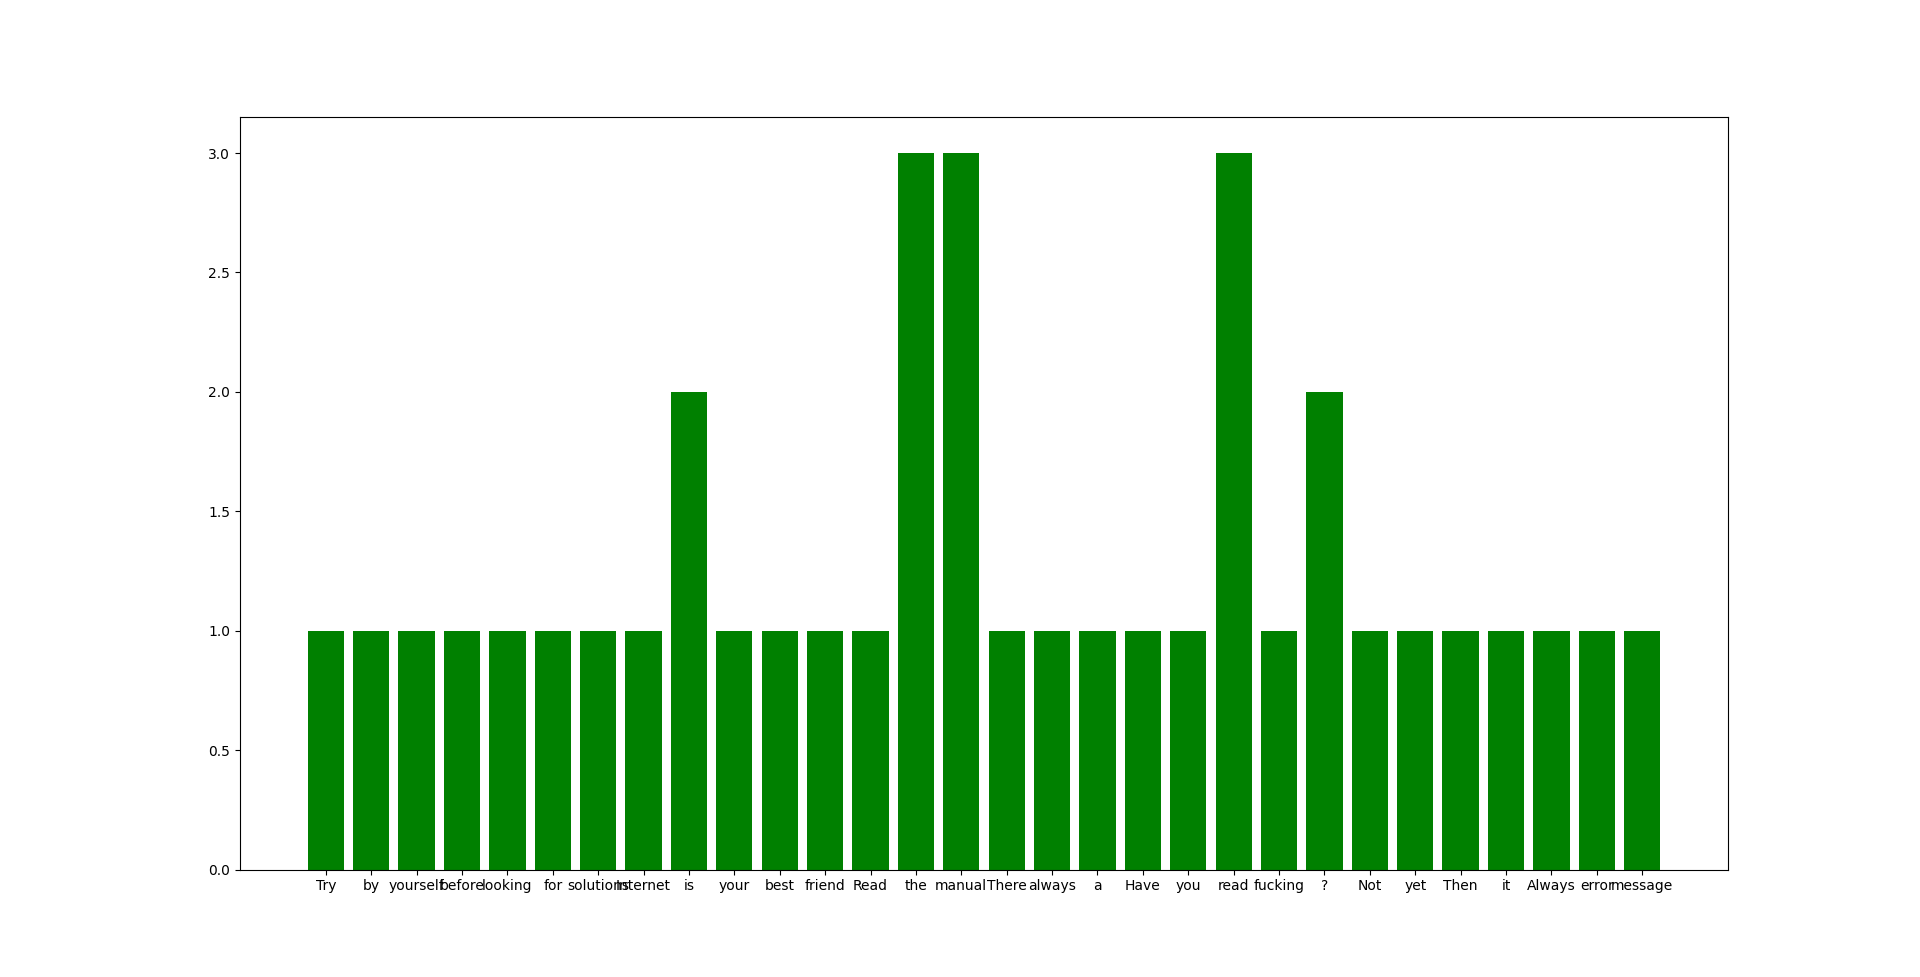
\includegraphics{hist.png}
\end{frame}

\end{document}
